\documentclass[a4paper,12pt]{ctexart}
\usepackage{graphicx}
\usepackage{geometry}
\geometry{left=2.5cm, right=2.5cm, top=2.5cm, bottom=2.5cm}
\usepackage{titlesec}
\usepackage{float}
\usepackage{caption}
\usepackage{hyperref}
\usepackage{xcolor}

\hypersetup{
    colorlinks=true,
    linkcolor=blue,
    filecolor=magenta,      
    urlcolor=cyan,
    pdftitle={商业计划书：菲兹旺德},
}

\title{\Huge \textbf{商业计划书}\\ \vspace{0.5cm} \Large 菲兹旺德—— 碳酸自由的魔法棒}
\author{太子瑞}
\date{\today}

\begin{document}

\maketitle
\thispagestyle{empty}
\newpage

\tableofcontents
\newpage

\section{一、 项目摘要 (Executive Summary)}
\textbf{FizzWand（中文名：菲兹旺德）}是一款首创的便携式物理去气搅拌装置。它通过微观多孔材料瞬间触发“成核反应”，让使用者能在数秒内优雅、高效地去除碳酸饮料中的气体。本项目致力于解决一个隐秘但广泛存在的痛点，结合便携性与时尚属性，打造一款属于年轻人的新潮 EDC（Everyday Carry，日常携带）单品。我们不仅销售工具，更在倡导一种“理解并照顾你的小习惯”的生活态度。目前已提交国家实用新型专利申请。

\section{二、 灵感与背景 (Inspiration \& Background)}
\subsection{1. 痛点发现：未被照顾的“小众”习惯}
在生活中，有这样一群人：
\begin{itemize}
    \item 他们因为肠胃敏感、容易胀气，而不敢大口畅饮冰镇汽水；
    \item 他们喜欢可乐或气泡水的甜味和香气，却极其讨厌气泡在口腔和喉咙里的刺激感；
    \item 他们曾试图用筷子狂搅、把杯子摇晃到喷溅，或者无奈地等汽水放到没气，只为了喝一口“没气的可乐”。
\end{itemize}
这似乎是一个“奇怪”甚至常被朋友取笑的小习惯。市面上没有任何一款产品专门为他们服务。我们发现，\textbf{这一需求不仅真实存在，而且因为长期被忽视，这类人群具有极高的忠诚度和痛点共鸣}。

\subsection{2. 命名灵感：FizzWand 菲兹旺德}
\begin{itemize}
    \item \textbf{Fizz}：英文中形容气泡嘶嘶冒出的声音，直击产品核心。
    \item \textbf{Wand}：魔杖。寓意着只需轻轻一点，魔法般瞬间让气泡消失。
    \item \textbf{菲兹旺德}：音译带来一种带有西方奇幻色彩的高级感，宛如魔法世界中不可或缺的随身法器。
\end{itemize}

\section{三、 技术原理与产品优势 (Technology \& Product)}
\subsection{1. 核心技术：成核反应 (Nucleation)}
FizzWand 摒弃了添加化学消泡剂的妥协，采用\textbf{纯物理方式}。其工作端由医疗级/食品级（316L/304）不锈钢粉末烧结而成，表面密布百万级微米孔（5$\mu m$ - 20$\mu m$）。

当魔棒插入碳酸饮料时，这些微孔提供了海量的\textbf{成核位点 (Nucleation sites)}。游离状态的二氧化碳分子迅速在这些位点聚集形成气泡并瞬间析出，如同将一颗薄荷糖投入可乐中一般剧烈，但\textbf{完全不改变饮料的任何风味}。抛光的手柄设计确保了气泡仅在底部爆发，防止液体顺杆喷溅。

\subsection{2. 核心优势}
\begin{itemize}
    \item \textbf{极速}：5-10秒内完成去气，比静置快数千倍。
    \item \textbf{无害}：纯物理过程，0添加，保留原味。
    \item \textbf{优雅}：告别疯狂摇晃的狼狈，动作从容如调酒师。
\end{itemize}

\section{四、 商业计划与产品线 (Business Plan \& Product Lines)}
FizzWand 的定位不仅是餐具，更是\textbf{时尚配饰与 EDC 装备}。

\subsection{1. 极致便携，随身相伴}
\begin{itemize}
    \item \textbf{尺寸设计}：整体长度控制在 15-18cm，直径 6mm，与一支高端钢笔无异。
    \item \textbf{收纳方案}：配备定制抗菌金属管套或真皮笔套，防漏防污，完美放入衬衫口袋或女士小挎包中，随时随地，想用就用。
\end{itemize}

\subsection{2. 时尚赋能，潮玩属性}
我们将打破传统餐具的刻板印象，赋予 FizzWand 情绪价值，打造系列化产品线：

\subsubsection*{（1）基础版 (Classic Edition)}
极简包豪斯风格，哑光金属杆身搭配金色多孔工作端。专为追求实用与极简美学的用户设计。

\begin{figure}[H]
    \centering
    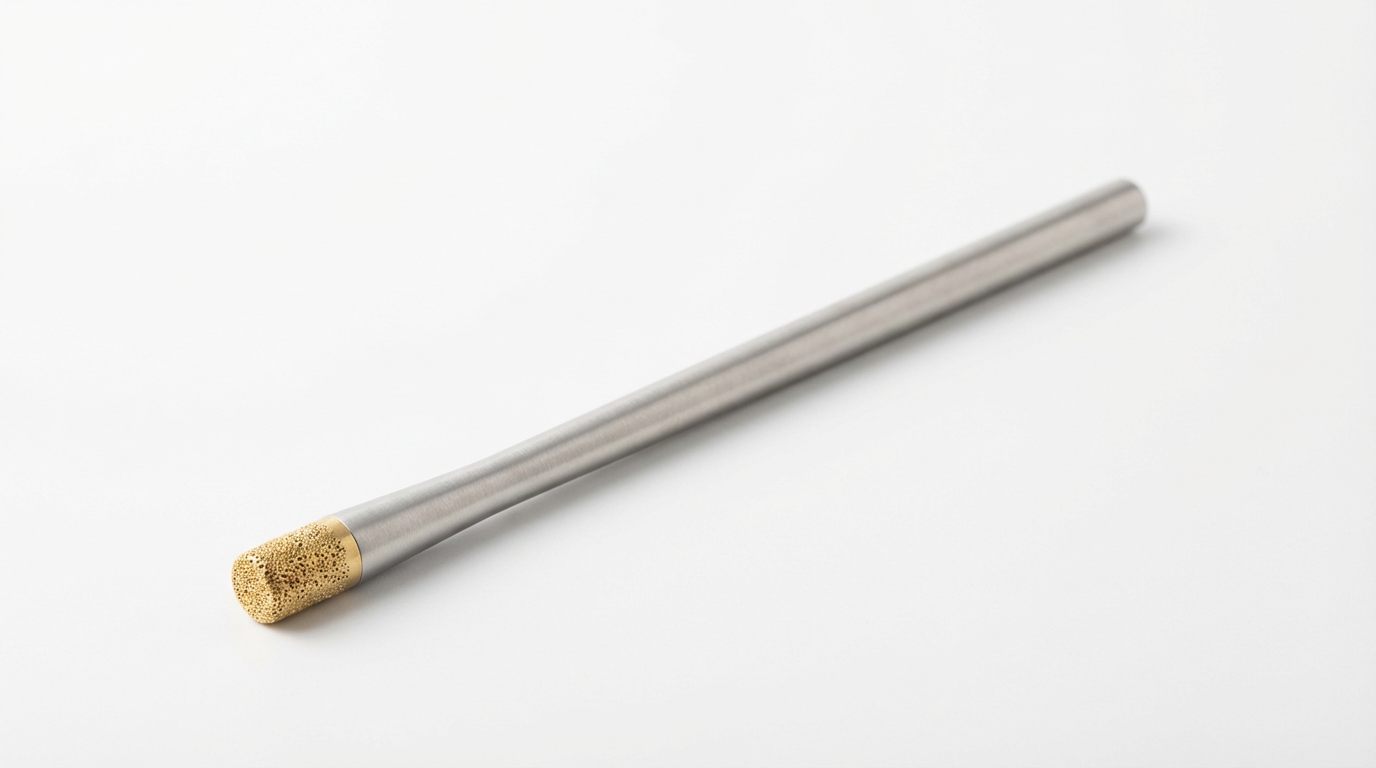
\includegraphics[width=0.6\textwidth]{fizzwand_classic.png}
    \caption{FizzWand 基础版 (Classic Edition) 概念图}
\end{figure}

\subsubsection*{（2）魔棒版 (Magic Wand Edition)}
将顶端多孔部分设计成\textbf{星型}，赋予挥舞魔杖的仪式感，直击年轻女性和二次元受众。只需轻轻一挥，即刻释放魔法。

\begin{figure}[H]
    \centering
    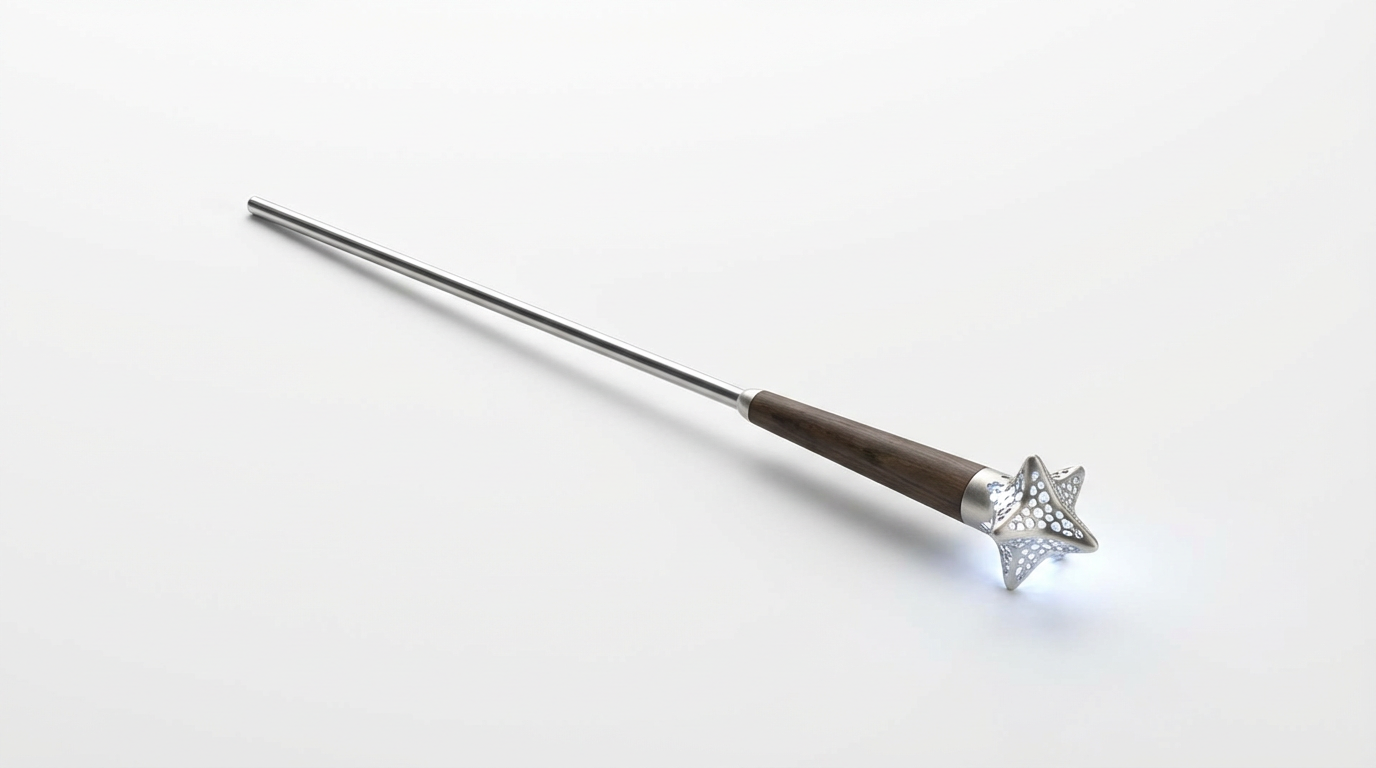
\includegraphics[width=0.6\textwidth]{fizzwand_magic.png}
    \caption{FizzWand 魔棒版 (Magic Wand Edition) 概念图}
\end{figure}

\subsubsection*{（3）雕塑版/高定版 (Artisan Edition)}
手柄部分融合经典艺术元素，例如以著名雕塑\textbf{《思考者》}为原型的金属或实木雕刻手柄。使其不仅是去气工具，更是餐桌上的艺术摆件和高档礼品。

\begin{figure}[H]
    \centering
    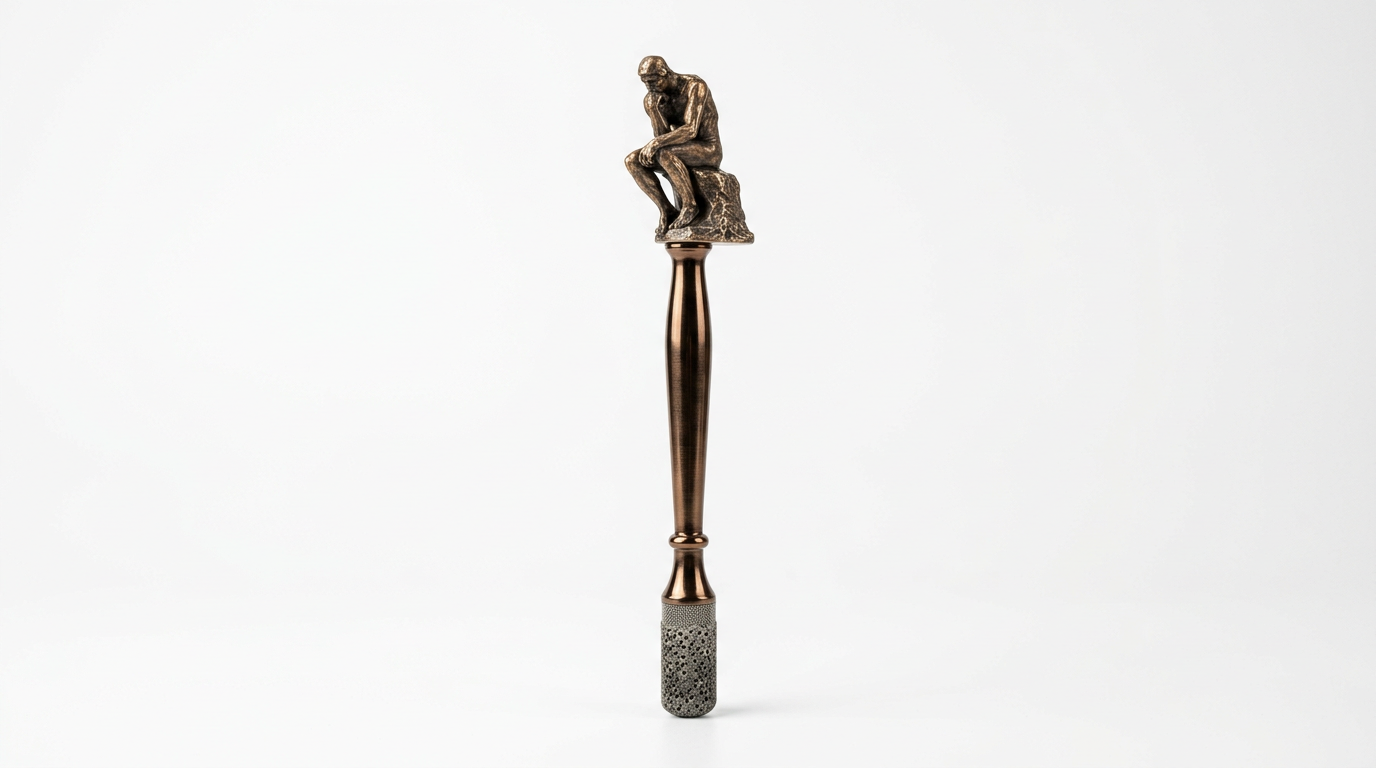
\includegraphics[width=0.6\textwidth]{fizzwand_thinker.png}
    \caption{FizzWand 雕塑版 - “思考者” (Artisan Edition) 概念图}
\end{figure}


\section{五、 营销与宣传策略 (Marketing Strategy)}
主打\textbf{DTC（Direct to Consumer，直接面对消费者）线上销售}模式，以极低的情绪成本撬动传播。

\subsection{1. 核心广告语（品牌态度）}
\begin{center}
    \Large \textbf{“FizzWand，理解您的小习惯。”} \\
    \large \textit{(FizzWand, We get your little quirks.)}
\end{center}

\subsection{2. 内容营销：共鸣与“被治愈”}
\begin{itemize}
    \item \textbf{痛点营销}：在小红书、抖音、B站发布短视频，重现那些因为“不喝带气的汽水”而被嘲笑的场景。FizzWand 作为“救星”出场，主打情绪共鸣：“你的小怪癖，在这里是被尊重的需求。”
    \item \textbf{视觉奇观（ASMR/解压）}：利用微距镜头拍摄 FizzWand 插入汽水瞬间，海量气泡如火山爆发般涌出，伴随密集的“嘶嘶”声。这种极度解压的视觉和听觉体验（ASMR）具有天然的病毒传播体质。
    \item \textbf{KOC 种草}：寻找那些有胃部困扰的博主、喜欢调饮的博主、以及 EDC 装备爱好者进行初期产品评测。
\end{itemize}

\subsection{3. 社群建立：隐藏者的狂欢}
建立“无气碳酸爱好者”社群。将一个原本隐藏的、弱势的小习惯，转化为一种专属的、酷的身份认同。

\section{六、 投资亮点 (Investment Highlights)}
\begin{enumerate}
    \item \textbf{空白市场}：真正的蓝海，目前市场上尚无针对此特定痛点的成熟物理去气竞品。
    \item \textbf{高毛利与复购}：产品结构精简，规模化生产后成本可控（粉末烧结工艺成熟）。丰富的版本（经典、星型、雕塑等）能持续拉高客单价并促成复购（收集癖）。
    \item \textbf{知识产权壁垒}：核心结构已申请国家实用新型专利，具备先发护城河。
    \item \textbf{强社交货币}：自带话题性，拿在手里、用在杯里，极易引发周围人的好奇与询问，自带裂变传播属性。
\end{enumerate}

\section{七、 融资规划与愿景 (Financial \& Vision)}
\subsection{1. 融资需求}
\textbf{本轮为种子轮融资，计划融资额：10万元人民币。}
\textbf{出让股权比例：30\%。}

\subsection{2. 资金用途}
\begin{itemize}
    \item \textbf{30\%（3万元）}：用于模具开发与首批产品（包括管套/皮套）的打样与小批量生产验证。
    \item \textbf{40\%（4万元）}：用于线上内容制作（高清晰度微距解压视频拍摄、产品精修图）与初期社交媒体精准投放（小红书、抖音）。
    \item \textbf{30\%（3万元）}：用于后续团队组建、知识产权全球布局（PCT国际专利申请准备）及日常运营备用金。
\end{itemize}

\subsection{3. 愿景}
让 FizzWand 成为全球数千万肠胃敏感者及无气饮料爱好者的口袋标配，将一个“怪癖”变成一种全新的生活方式！

\end{document}